\documentclass[12pt]{article}

%packages
\usepackage[brazil]{babel}
\usepackage[utf8]{inputenc}
\usepackage[usenames,dvipsnames,svgnames,table]{xcolor}
\usepackage[a4paper,margin={1in}]{geometry}
\usepackage{graphicx}
\usepackage{indentfirst}
\usepackage{subcaption}
\usepackage{url}



%% Pulando linhas
\renewcommand{\baselinestretch}{1.5}

\newcommand{\vsp}{\vspace{0.2in}}

\begin {document}
	
	
	\centerline{
		\begin{minipage}[t]{5in}
			\begin{center}
				{\Large \bf Tarefa: implementação de convolução e correlação}
				\vsp \\
				{\small {\bf Disciplina:} Análise e Reconhecimento de Formas - MAC5749 / IME-USP}\\
				{\small {\bf Professor:} Roberto Marcondes Cesar Jr.}
			\end{center}
		\end{minipage}
	}
	\vsp

\section{Implementação}
O código está disponível no arquivo \textbf{exercicio1.py} e foi implementado em linguagem Python. Para o cálculo das operações de convolução e correlação foi utilizada a biblioteca científica \textit{Numpy}. Já para a construção dos gráficos das funções, foi utilizada a biblioteca \textit{Matplotlib}.

\section{Gráficos}

\subsection{Definições}
\begin{figure}[h]
	\centering
	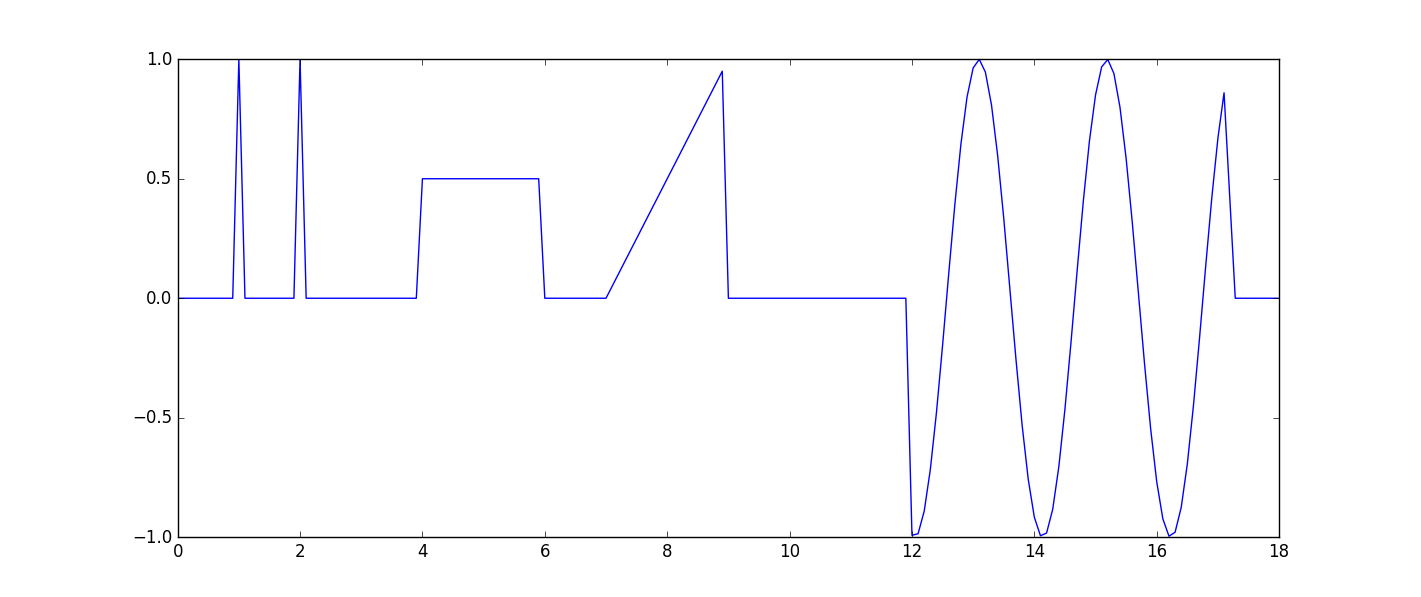
\includegraphics[width=1.05\linewidth]{h.png}
	\caption{gráfico da função $h(t)$}
	\label{fig:h}
\end{figure}
\clearpage

\begin{figure}[!h]
	\centering
	\begin{minipage}[b]{0.49\linewidth}
		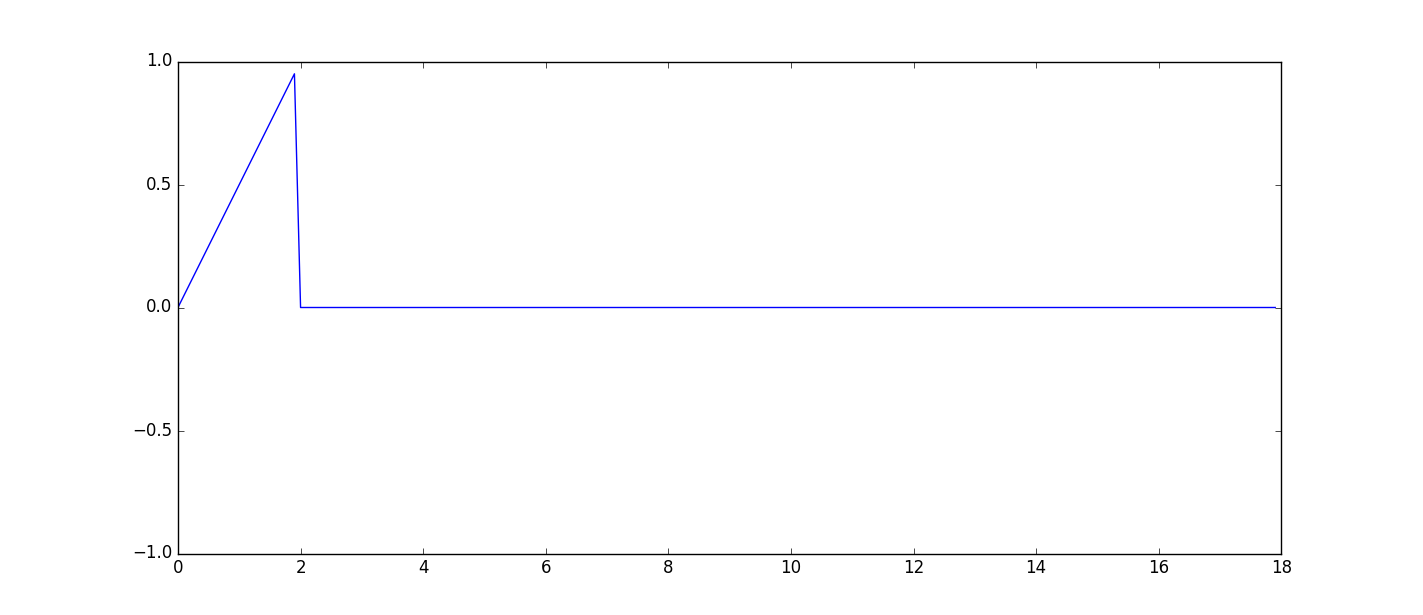
\includegraphics[width=1.15\linewidth]{g1.png}
		\caption{gráfico da função rampa $g_1(t)$}
	\end{minipage}
	\hfill
	\begin{minipage}[b]{0.49\linewidth}
		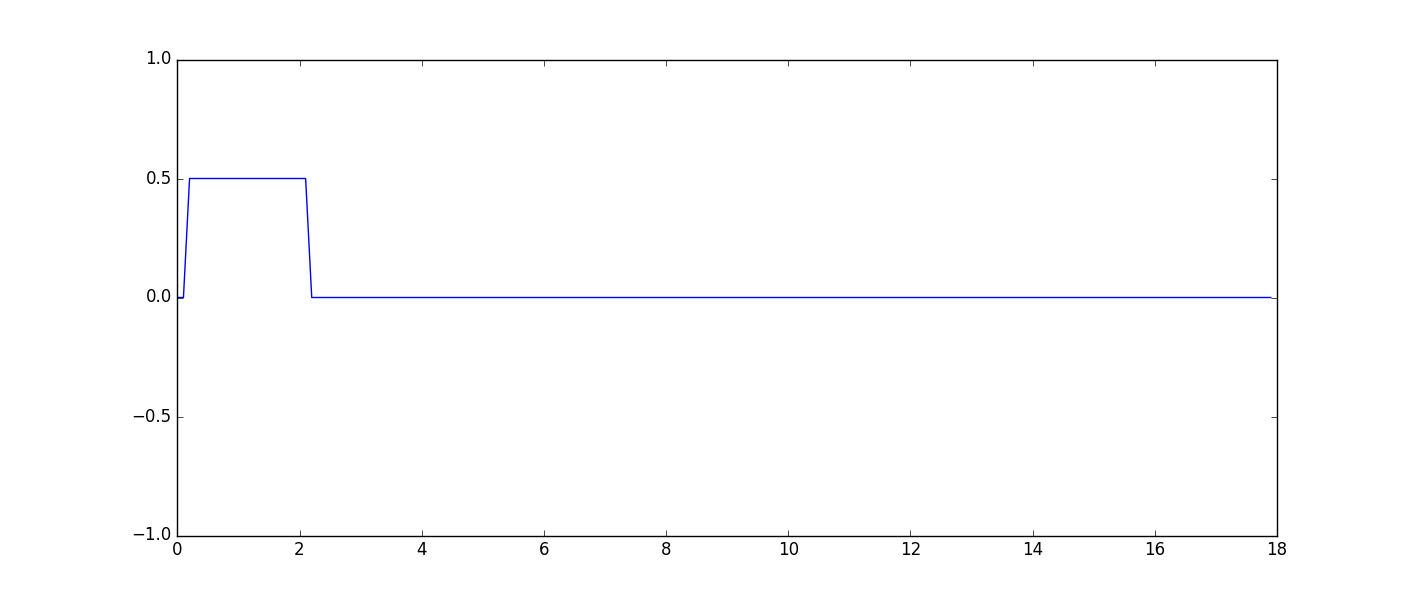
\includegraphics[width=1.15\linewidth]{g2.png}
		\caption{gráfico da função platô $g_2(t)$}
	\end{minipage}
	\vspace{1cm}
	
	\begin{minipage}[b]{0.49\linewidth}
		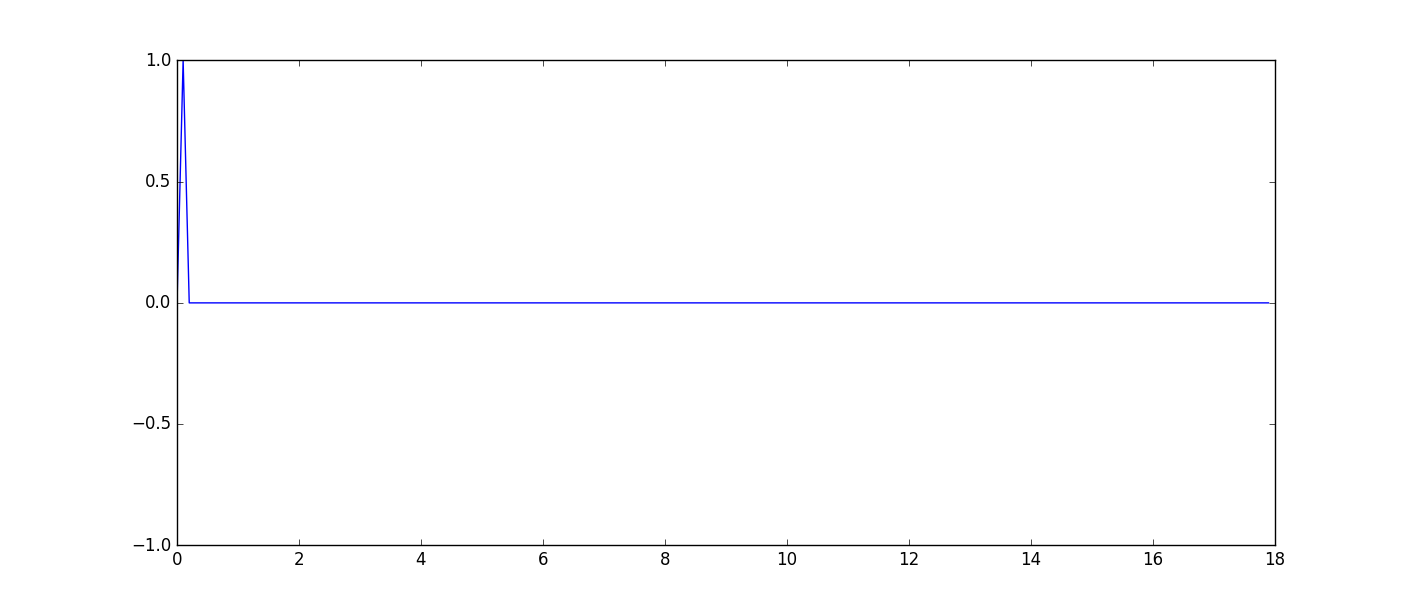
\includegraphics[width=1.15\linewidth]{g3.png}
		\caption{gráfico da função pulso $g_3(t)$}
	\end{minipage}
	\hfill
	\begin{minipage}[b]{0.49\linewidth}
		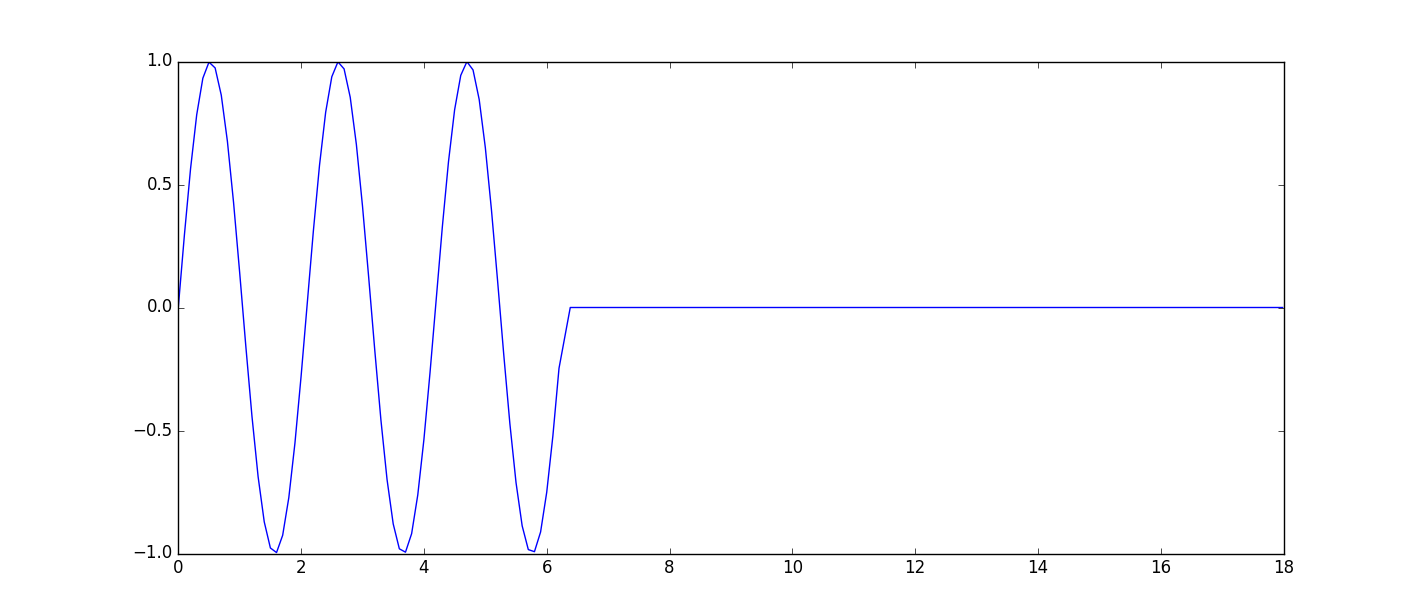
\includegraphics[width=1.15\linewidth]{g4.png}
		\caption{gráfico da função seno $g_4(t)$}
	\end{minipage}
\end{figure}

	
\subsection{Operações de convolução}

\begin{figure}[!h]
	\centering
	\begin{minipage}[b]{0.49\linewidth}
		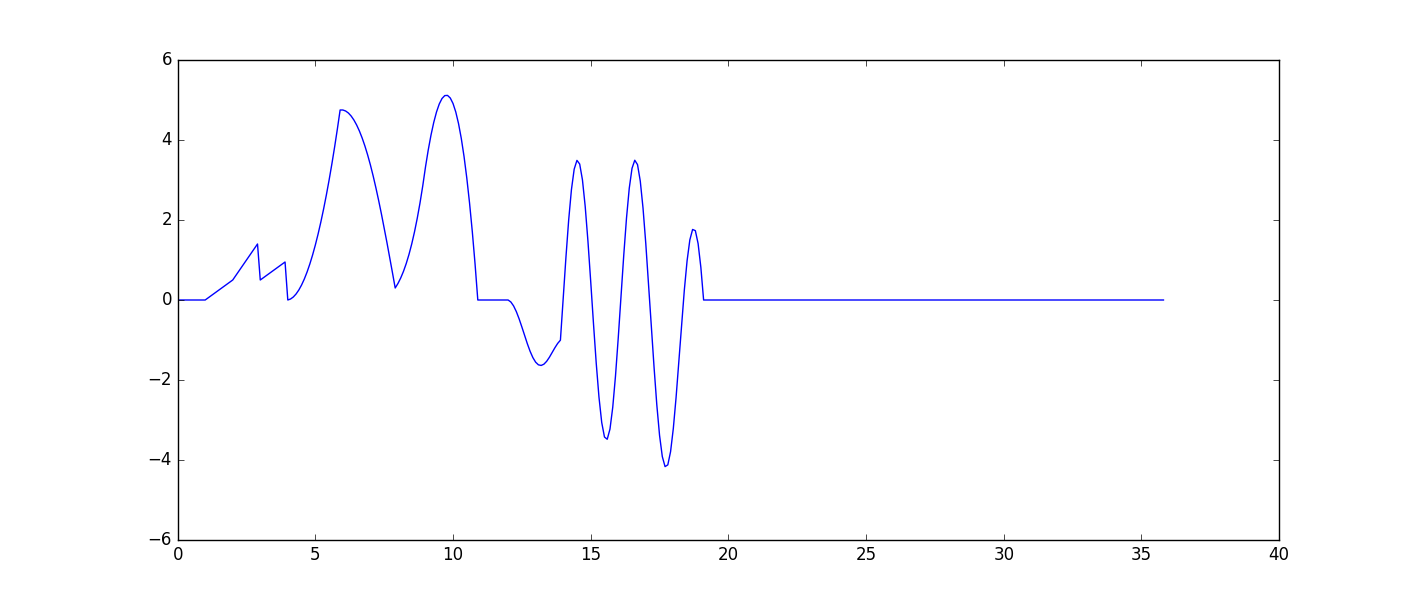
\includegraphics[width=1.15\linewidth]{h*g1.png}
		\caption{gráfico de $(h*g_1)(t)$}
	\end{minipage}
	\hfill
	\begin{minipage}[b]{0.49\linewidth}
		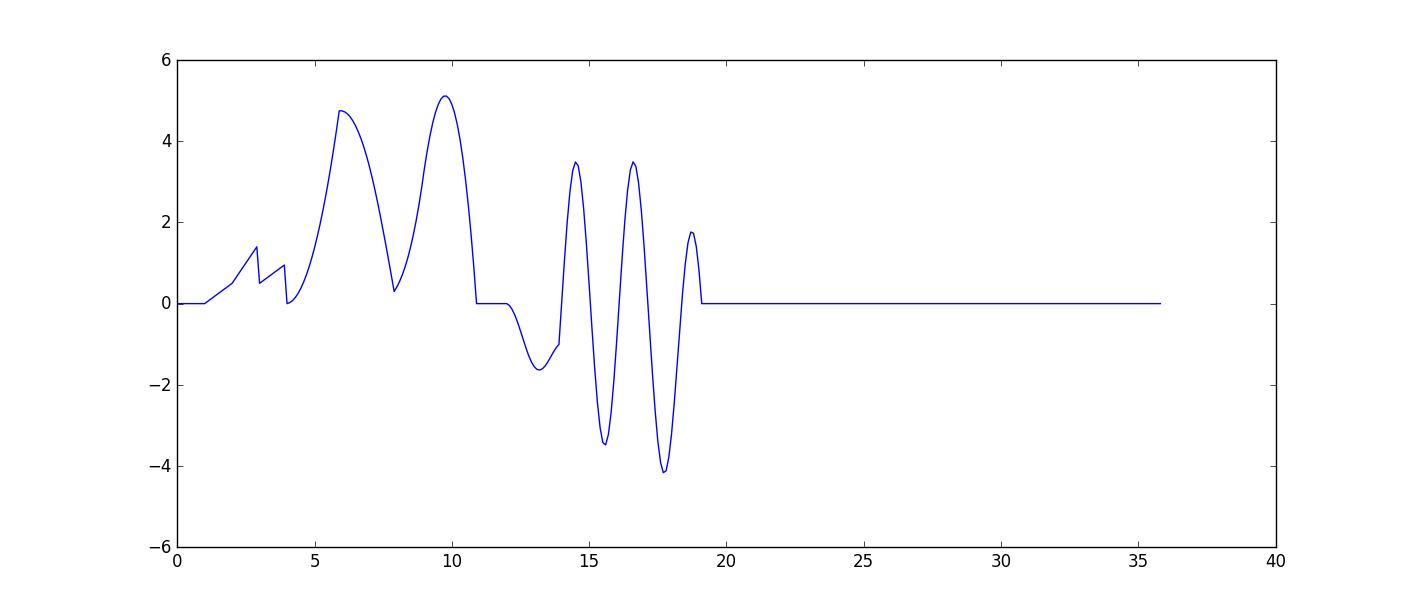
\includegraphics[width=1.15\linewidth]{g1*h.png}
		\caption{gráfico de $(g_1*h)(t)$}
	\end{minipage}
\end{figure}

\begin{figure}[!h]
	\centering
	\begin{minipage}[b]{0.49\linewidth}
		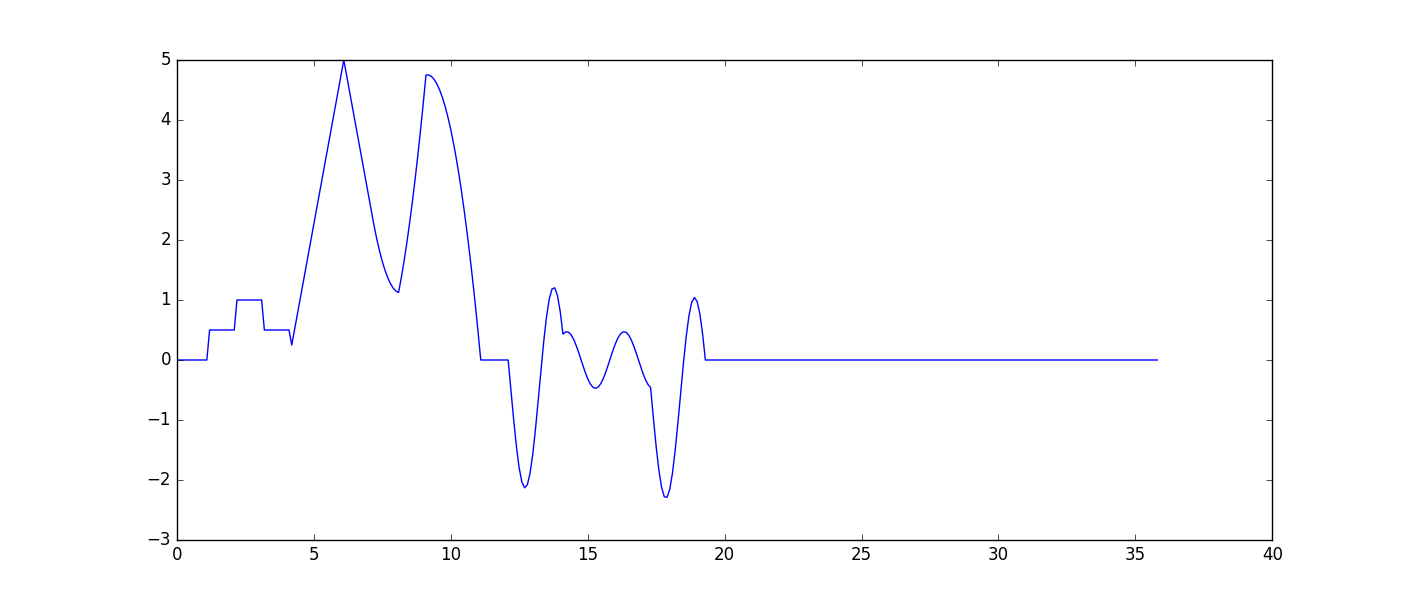
\includegraphics[width=1.15\linewidth]{h*g2.png}
		\caption{gráfico de $(h*g_2)(t)$}
	\end{minipage}
	\hfill
	\begin{minipage}[b]{0.49\linewidth}
		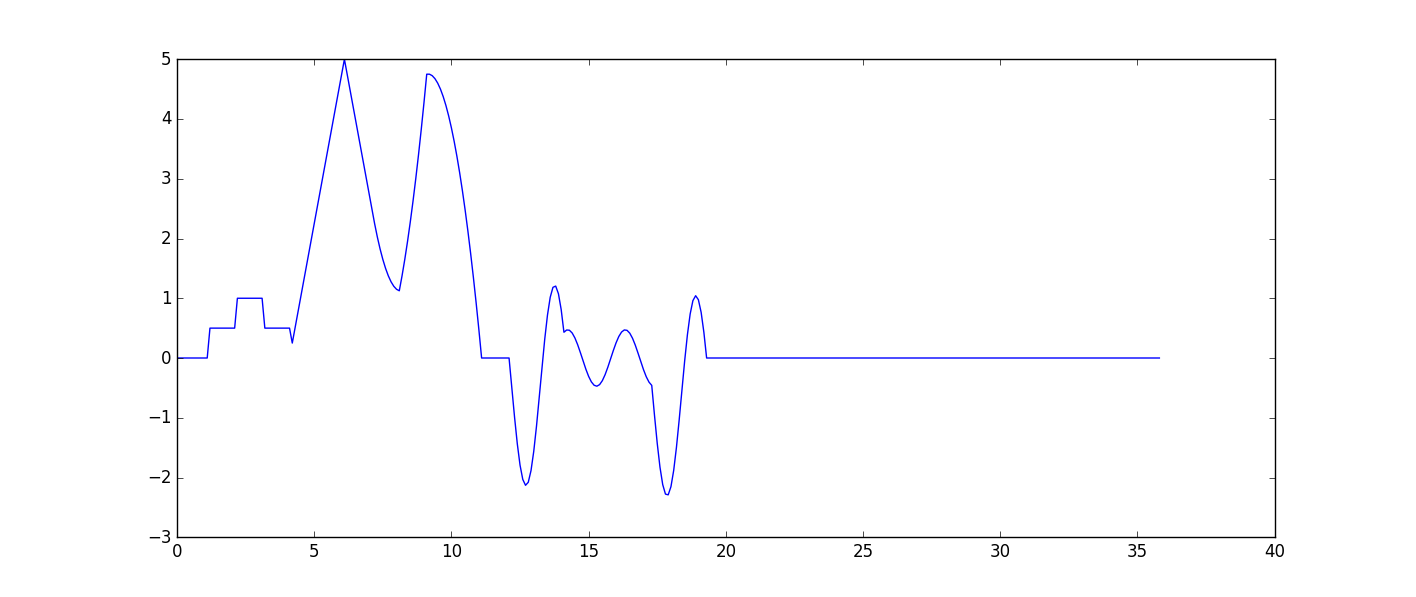
\includegraphics[width=1.15\linewidth]{g2*h.png}
		\caption{gráfico de $(g_2*h)(t)$}
	\end{minipage}
\end{figure}

\begin{figure}[!h]
	\centering
	\begin{minipage}[b]{0.49\linewidth}
		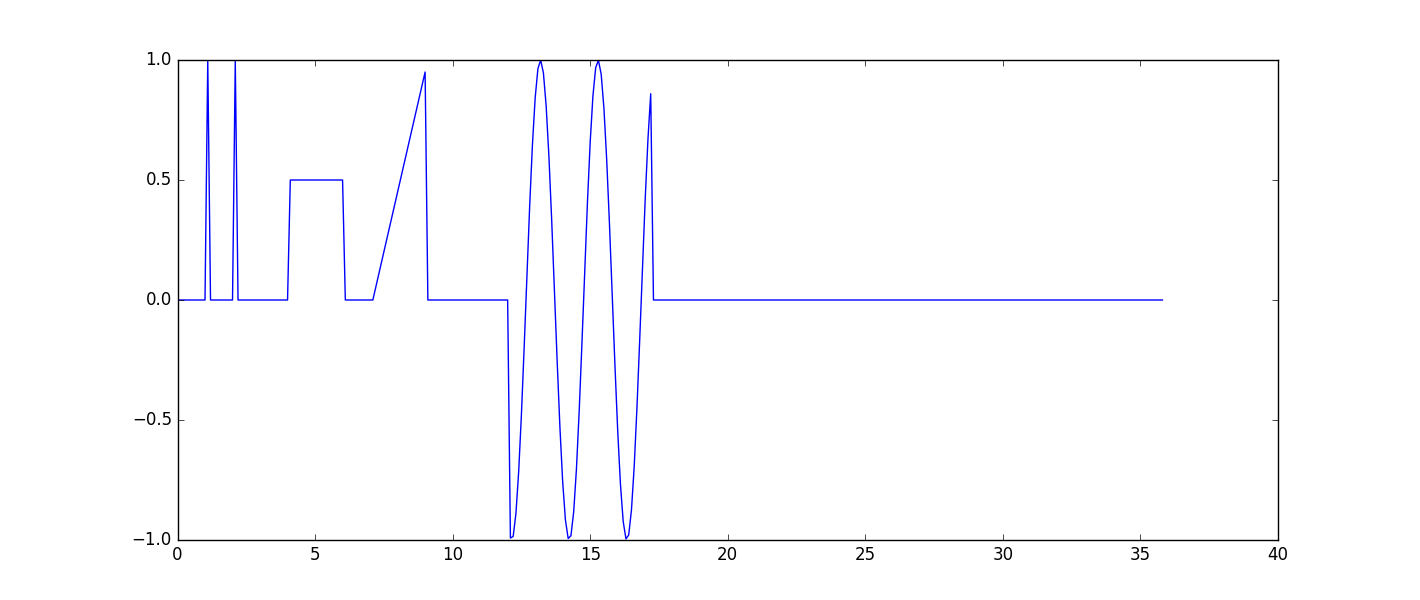
\includegraphics[width=1.15\linewidth]{h*g3.png}
		\caption{gráfico de $(h*g_3)(t)$}
	\end{minipage}
	\hfill
	\begin{minipage}[b]{0.49\linewidth}
		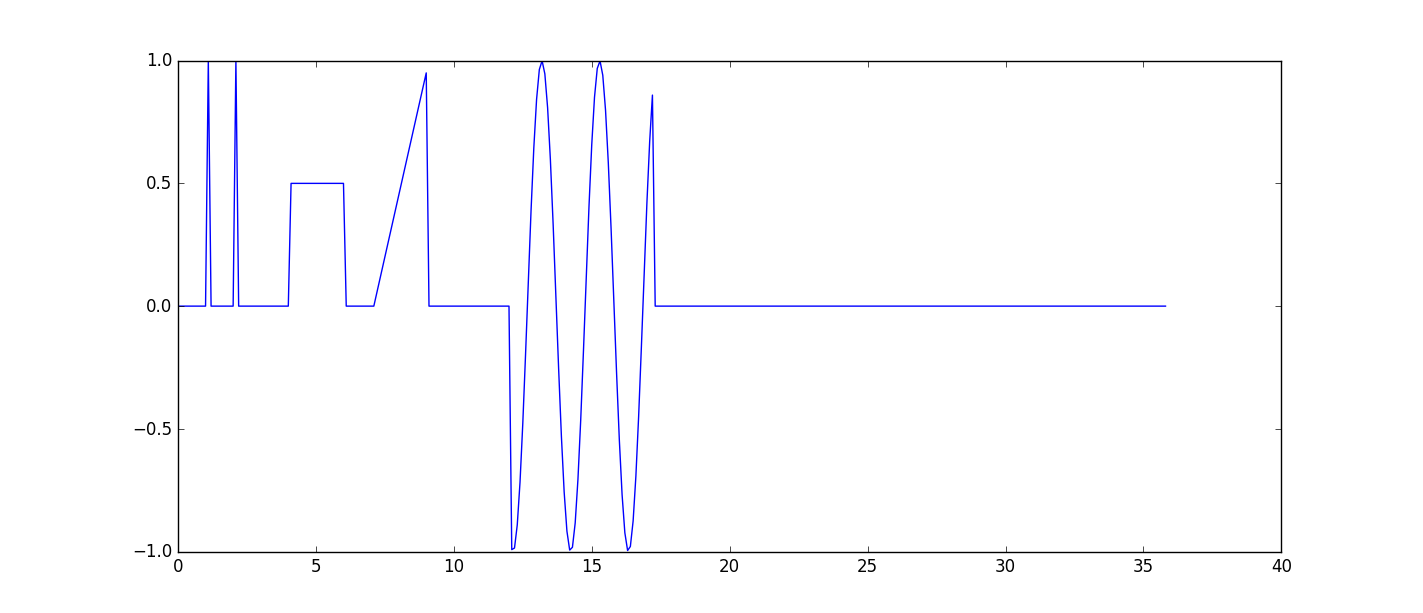
\includegraphics[width=1.15\linewidth]{g3*h.png}
		\caption{gráfico de $(g_3*h)(t)$}
	\end{minipage}
\end{figure}

\begin{figure}[!h]
	\centering
	\begin{minipage}[b]{0.49\linewidth}
		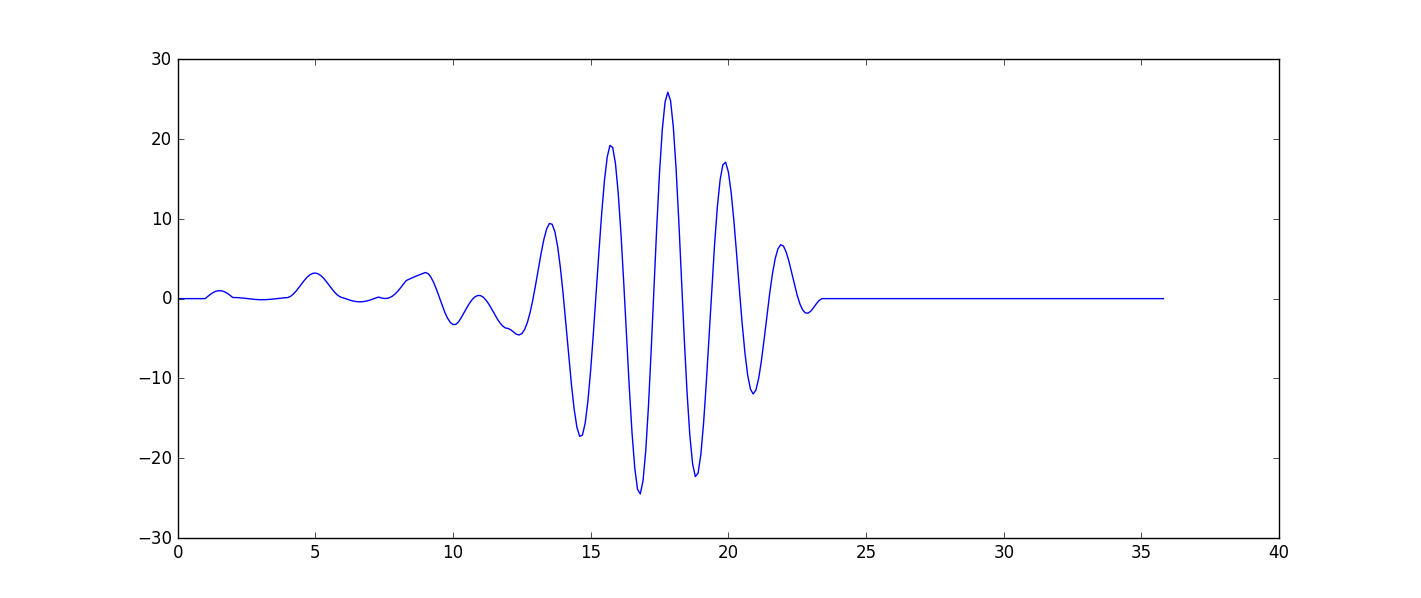
\includegraphics[width=1.15\linewidth]{h*g4.png}
		\caption{gráfico de $(h*g_4)(t)$}
	\end{minipage}
	\hfill
	\begin{minipage}[b]{0.49\linewidth}
		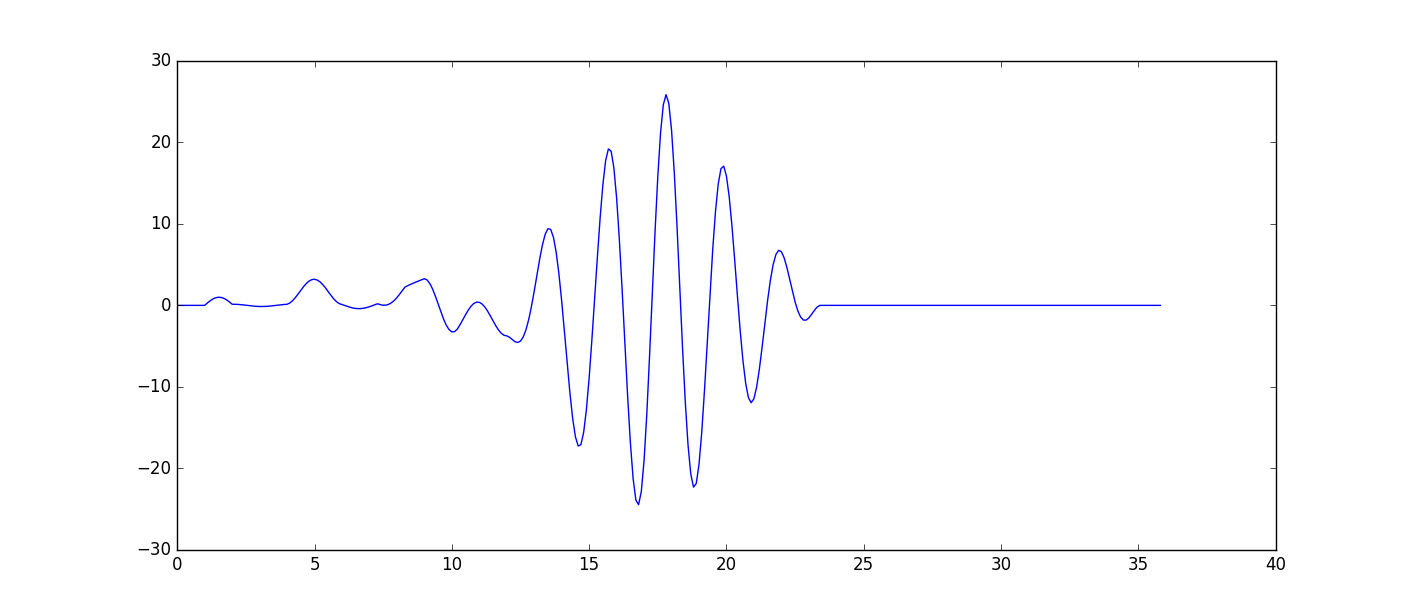
\includegraphics[width=1.15\linewidth]{g4*h.png}
		\caption{gráfico de $(g_4*h)(t)$}
	\end{minipage}
\end{figure}
\clearpage

\subsection{Operações de correlação}

\begin{figure}[!h]
	\centering
	\begin{minipage}[b]{0.49\linewidth}
		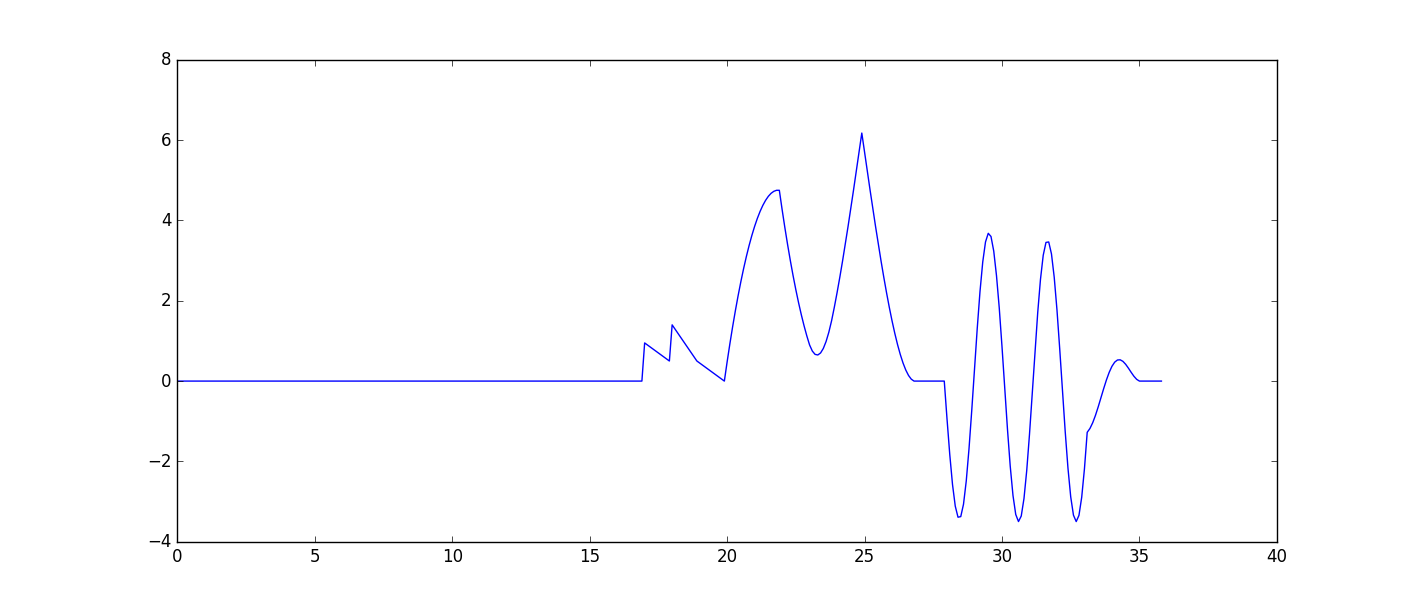
\includegraphics[width=1.15\linewidth]{hog1.png}
		\caption{gráfico de $(h\circ g_1)(t)$}
	\end{minipage}
	\hfill
	\begin{minipage}[b]{0.49\linewidth}
		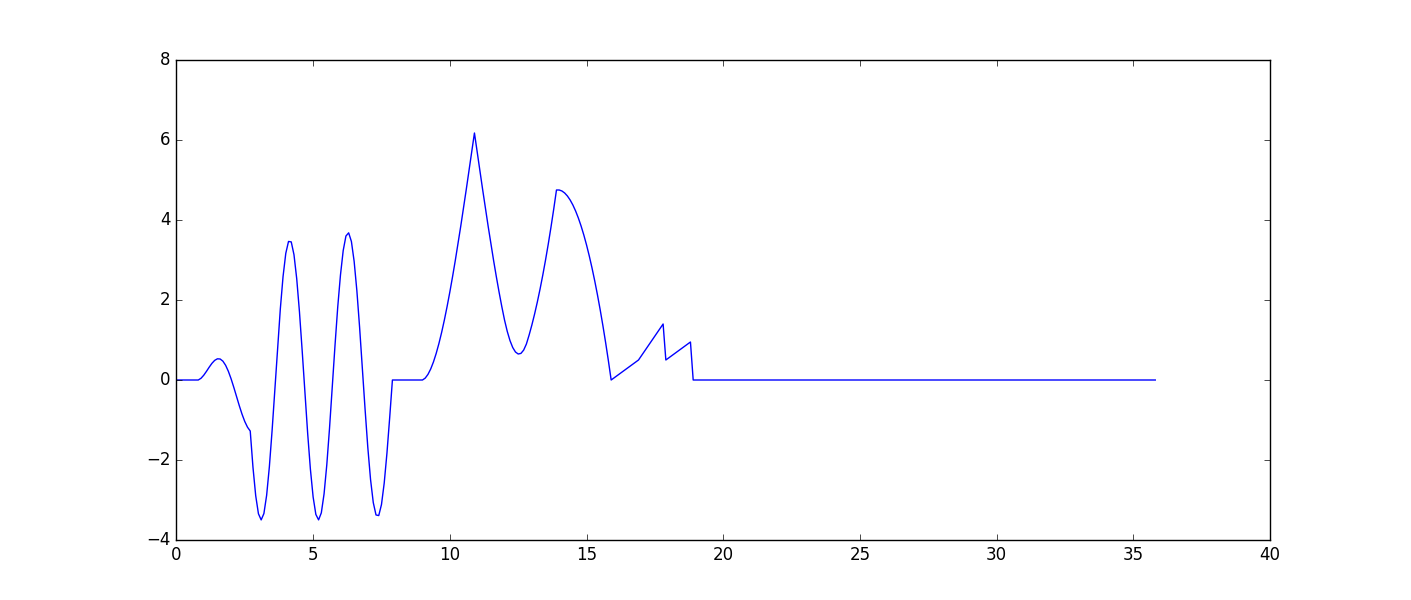
\includegraphics[width=1.15\linewidth]{g1oh.png}
		\caption{gráfico de $(g_1\circ h)(t)$}
	\end{minipage}
\end{figure}

\begin{figure}[!h]
	\centering
	\begin{minipage}[b]{0.49\linewidth}
		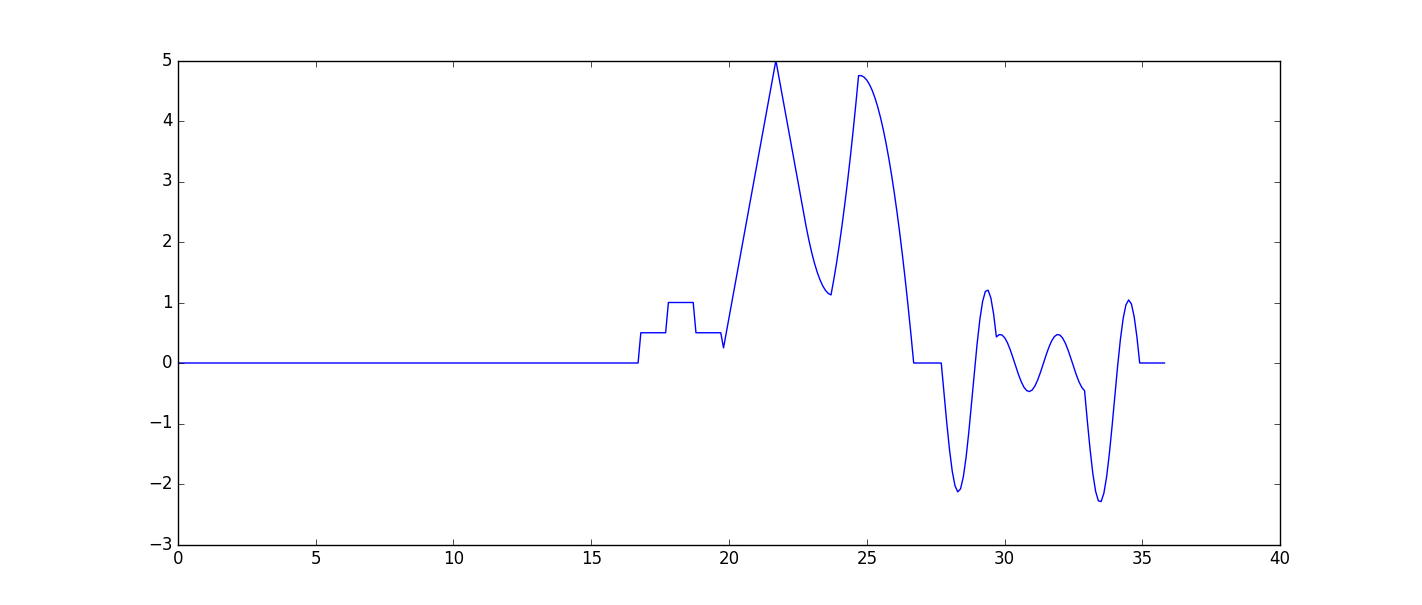
\includegraphics[width=1.15\linewidth]{hog2.png}
		\caption{gráfico de $(h\circ g_2)(t)$}
	\end{minipage}
	\hfill
	\begin{minipage}[b]{0.49\linewidth}
		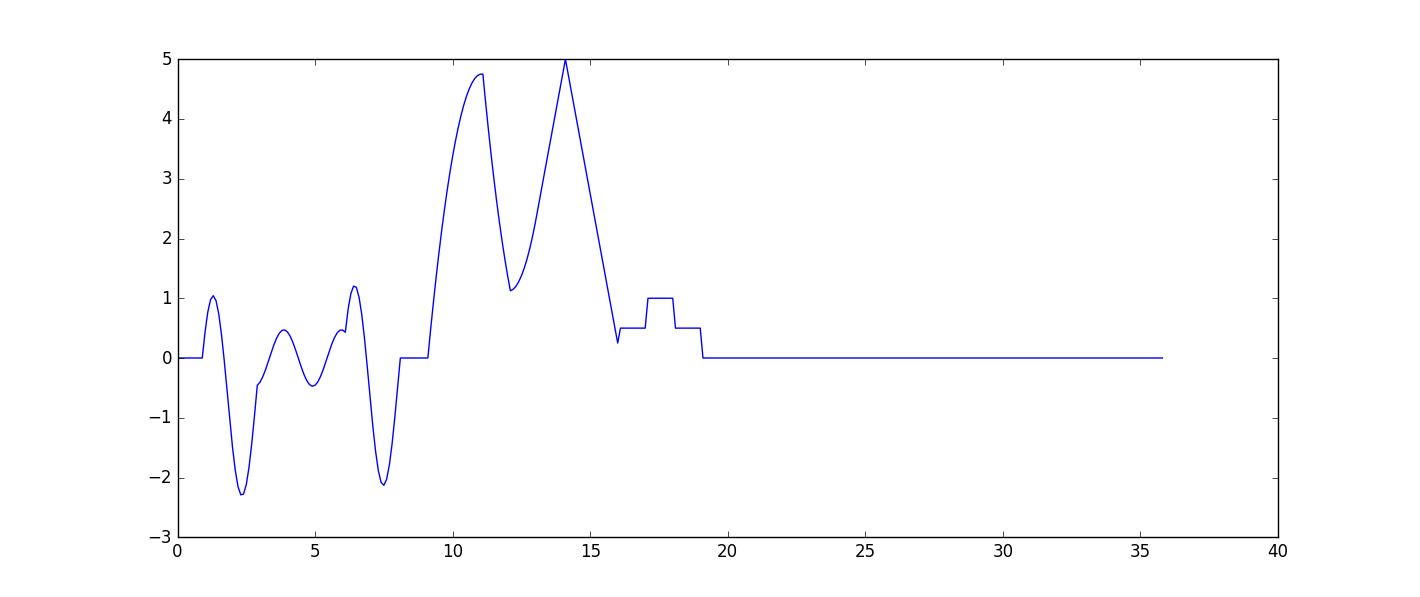
\includegraphics[width=1.15\linewidth]{g2oh.png}
		\caption{gráfico de $(g_2\circ h)(t)$}
	\end{minipage}
\end{figure}

\begin{figure}[!h]
	\centering
	\begin{minipage}[b]{0.49\linewidth}
		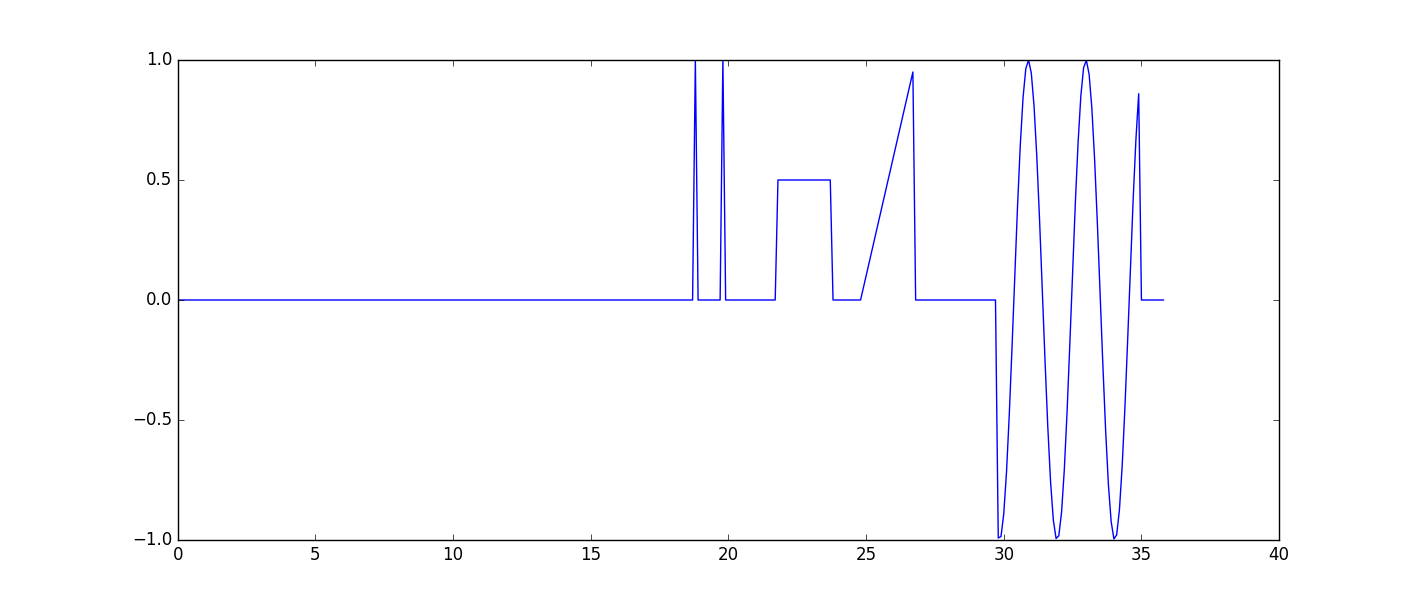
\includegraphics[width=1.15\linewidth]{hog3.png}
		\caption{gráfico de $(h\circ g_3)(t)$}
	\end{minipage}
	\hfill
	\begin{minipage}[b]{0.49\linewidth}
		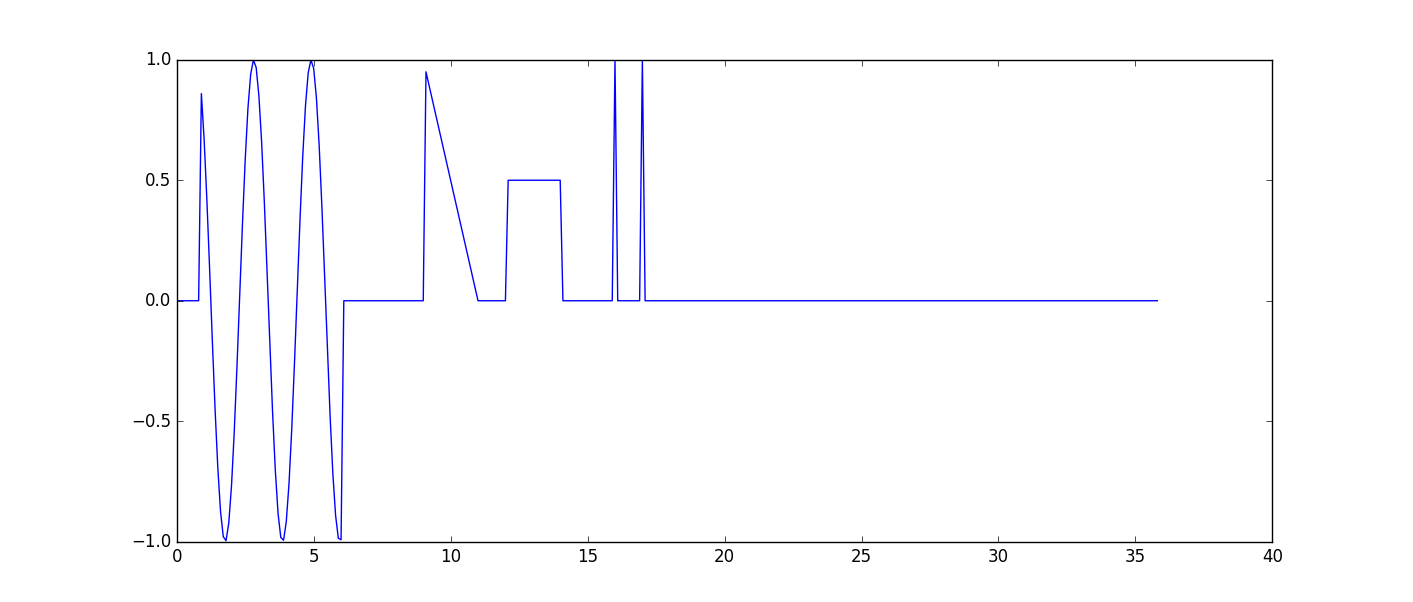
\includegraphics[width=1.15\linewidth]{g3oh.png}
		\caption{gráfico de $(g_3\circ h)(t)$}
	\end{minipage}
\end{figure}

\begin{figure}[!h]
	\centering
	\begin{minipage}[b]{0.49\linewidth}
		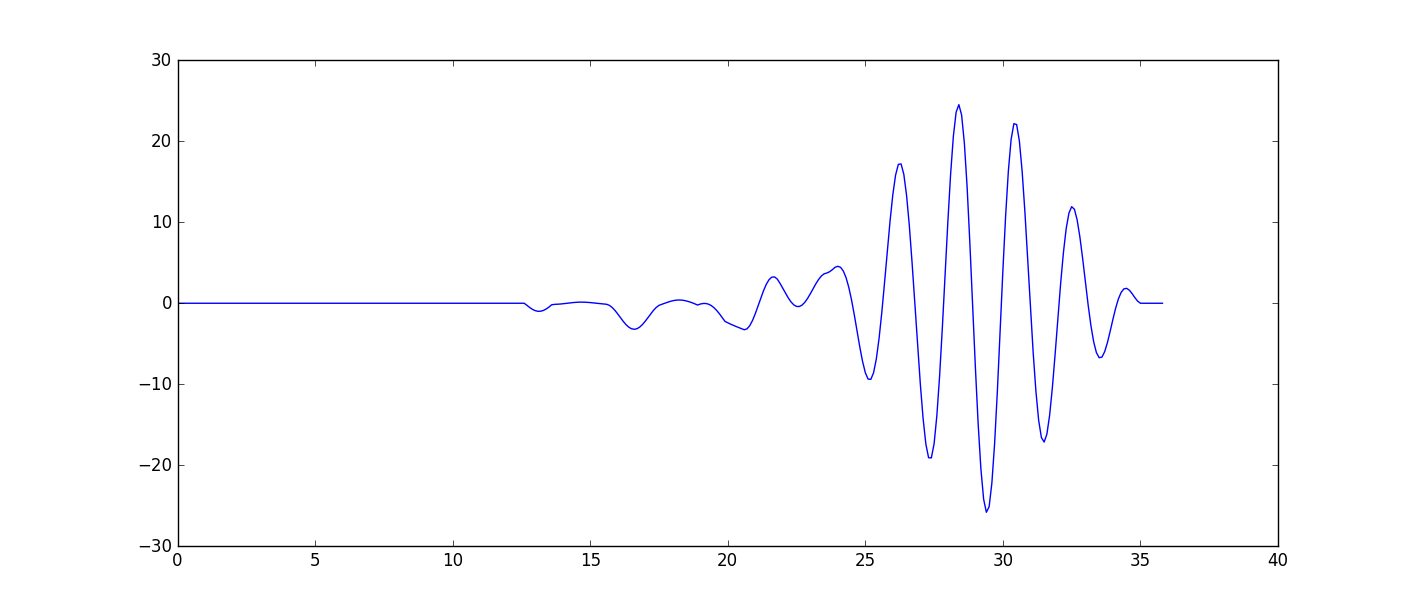
\includegraphics[width=1.15\linewidth]{hog4.png}
		\caption{gráfico de $(h\circ g_4)(t)$}
	\end{minipage}
	\hfill
	\begin{minipage}[b]{0.49\linewidth}
		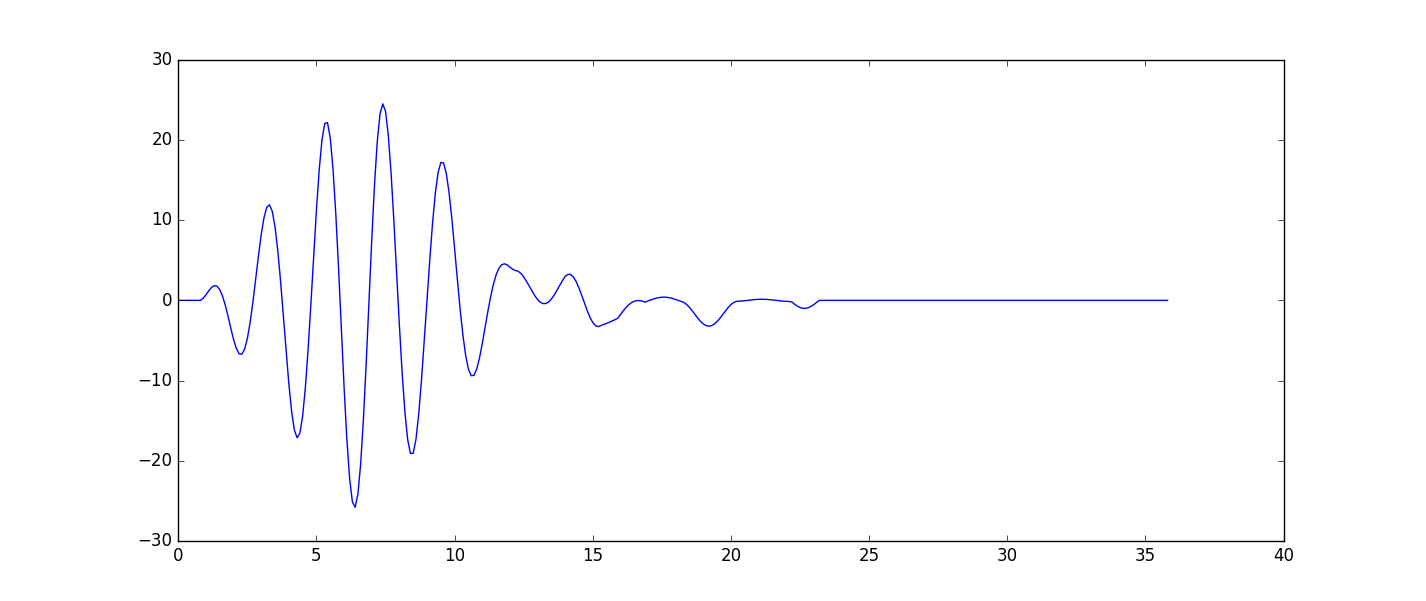
\includegraphics[width=1.15\linewidth]{g4oh.png}
		\caption{gráfico de $(g_4\circ h)(t)$}
	\end{minipage}
\end{figure}

\section{Interpretação}

\subsection{Resultados da convolução}
Um primeiro fato que pode ser depreendido dos gráficos gerados é que o sinal resultante de uma convolução é invariante à ordem com que os sinais de entrada convoluem.

No caso da convolução de $h$ com $g_1$, podemos observar que a interação de $g_1(\tau-t)$ com os dois pulsos no início de $h$ tende a formar um sinal semelhante à entrada $g_1$, conforme o valor de $\tau$ é incrementado, dado que a rampa é invertida na convolução. No entanto, a reprodução não é perfeita, uma vez que os pulsos estão muito próximos, provocando interferência no resultado. Em relação à interação de $g_1$ com o platô, podemos ver um sinal resultante simétrico, como esperado. Já quanto à rampa presente em $h$, notamos que no casamento com $g_1$ o sinal resultante é máximo. Em relação à interação com o seno presente em $h$, os trechos semelhantes são atenuados pela participação de valores negativos em $h$.

Na convolução entre $h$ e $g_2$, notamos que a reflexão de $g_2$ não é relevante para o resultado, dado que o sinal é simétrico. Percebemos ainda que a interação de $g_2$ com os pulsos de $h$ produz uma ``escada'', uma vez que ambos contribuem simultaneamente por um determinado intervalo no sinal resultante. Como esperado, o pico máximo ocorre no encaixe de $g_2$ com o platô de $h$, enquanto o seno fica bastante atenuado pela presença concomitante de valores positivos e negativos nos trechos cobertos por $g_2$.

No caso de $h$ com $g_3$, o resultado é consistente com a teoria. Como $g_3$ se comporta quase como um \textit{$\delta$ de Dirac}, decorre que o sinal resultante é o próprio $h$, pois tudo o que está sendo feito na prática é multiplicar cada ponto da função por uma unidade.

Por fim, na convolução entre $h$ e $g_4$, percebemos o efeito atenuador da interação de um sinal periódico com sinais não periódicos. Novamente, o ponto máximo da convolução se dá quando há um casamento entre $g_4$ e o seno contido em $h$.



\subsection{Resultados da correlação}
Na correlação, ao contrário da convolução, não há comutatividade. No entanto, como os valores de $g_i$ e $h$ são reais, vale que $(g_i \circ h)(\tau) = (h \circ g_i)(-\tau)$, o que pode ser observado nos gráficos gerados. Além disso, na correlação o sinal deslocado por $\tau$ não é invertido como na convolução, o que implica uma aparente inversão de direção no sinal resultante.

Assim, em comparação com a convolução, as correlações entre os sinais $g_i$ com $h$ não apresentam nenhuma outra característica particular além das já mencionadas. Talvez a única exceção seja a correlação entre $g_1$ e $h$. Nesse caso, além de observarmos o efeito de ``mudança de direção'' na interação da rampa com os pulsos de $h$, o fato de $g_1$ não ter o sinal invertido na correlação faz com que o casamento entre $g_1$ e a rampa contida em $h$ gere uma forma distinta em comparação com a convolução, isto é, um pico simétrico. 





\end{document}
